\documentclass[a4paper,12pt]{article}
\usepackage{latexsym}
\usepackage{graphicx}
\usepackage{epsfig}
\usepackage{float}
\usepackage{natbib}
\usepackage{listings}
\usepackage{amsmath}
\usepackage{gensymb}
\graphicspath{{./}}
\DeclareGraphicsExtensions{.jpg}
\author{Howard Kinsman}
\title{Cosmology Tutorial 9}
\begin{document}
\maketitle
\section{}
\subsection{}
In the radiation era fluctuations are frozen into a high density radiation field.
\begin{table}[ht]
\centering
\begin{tabular}{|l|l|l|}
\hline
Radiation & Plasma & Neutral \\
\hline
= & = & + \\
= & = & + \\
= & + & + \\
\hline
\end{tabular}
\caption{\label{tab:task1}Baryonic Isothermal}
\end{table}
\subsection{}
Silk damping occurs in the radiation era but Silk mass is reduced after decoupling.
\begin{table}[ht]
\centering
\begin{tabular}{|l|l|l|}
\hline
Radiation & Plasma & Neutral \\
\hline
- & - & + \\
+ & + & + \\
+ & + & + \\
\hline
\end{tabular}
\caption{\label{tab:task2}Baryonic Adiabatic}
\end{table}
\subsection{}
Fluctuations on small scales remain undamped.
\begin{table}[ht]
\centering
\begin{tabular}{|l|l|l|}
\hline
Radiation & Plasma & Neutral \\
\hline
+ & + & + \\
- & + & + \\
- & + & + \\
\hline
\end{tabular}
\caption{\label{tab:task3}CDM}
\end{table}
\subsection{}
Damping occurs due to free-streaming when particles are relativistic before $t_{eq}$.
\begin{table}[ht]
\centering
\begin{tabular}{|l|l|l|}
\hline
Radiation & Plasma & Neutral \\
\hline
- & + & + \\
- & + & + \\
- & + & + \\
\hline
\end{tabular}
\caption{\label{tab:task4}HDM}
\end{table}

\section{}
\begin{flalign*}
& k_x=n_x\frac{2\pi}{100} &\\
& 2\frac{2\pi}{100}=.126 &\\
& 3\frac{2\pi}{100}=.188 &\\
\end{flalign*}
so $n_x$ must be either 0,2 or 3. The wavelengths are:
\begin{flalign*}
& \frac{2\pi}{2}=\pi &\\
& \frac{2\pi}{3}=2.094 &\\
\end{flalign*}
There are $3^3=27$ permutations of $n_x$, $n_y$ and $n_z$.
For $1<k<2$ the interval is 10 times larger so presumably there are 10 times as many permutations i.e. 270?
.
\section{}
\subsection{}
The Horizon scale at matter-energy equality is approximately 100 Mpc. The amplitude of fluctuations is $\approx10^{-4}$.
\subsection{}
\begin{table}[ht]
\centering
\begin{tabular}{|l|l|l|l|}
\hline
Redshift & Amplitude & Log(Amplitude) & Log(a) \\
\hline
$4\times10^{7}$ & $10^{-8}$ & -8 & -7.6 \\
$6.6\times10^{6}$ & $10^{-7}$ & -7 & -6.8 \\
$2.2\times10^{6}$ & $10^{-6}$ & -6 & -6.3 \\
$1.4\times10^{6}$ & $10^{-5}$ & -5 & -6.1 \\
$6.3\times10^{5}$ & $10^{-4}$ & -4 & -5.7 \\
39000 & $10^{-3}$ & -3 & -4.6 \\
490 & $.01$ & -2 & -2.7 \\
29 & $.1$ & -1 & -1.5 \\
$2.2$ & $1$ & 0 & -0.5 \\
\hline
\end{tabular}
\caption{\label{tab:task6}Question 3 data}
\end{table}
\begin{figure}[H]
\centering
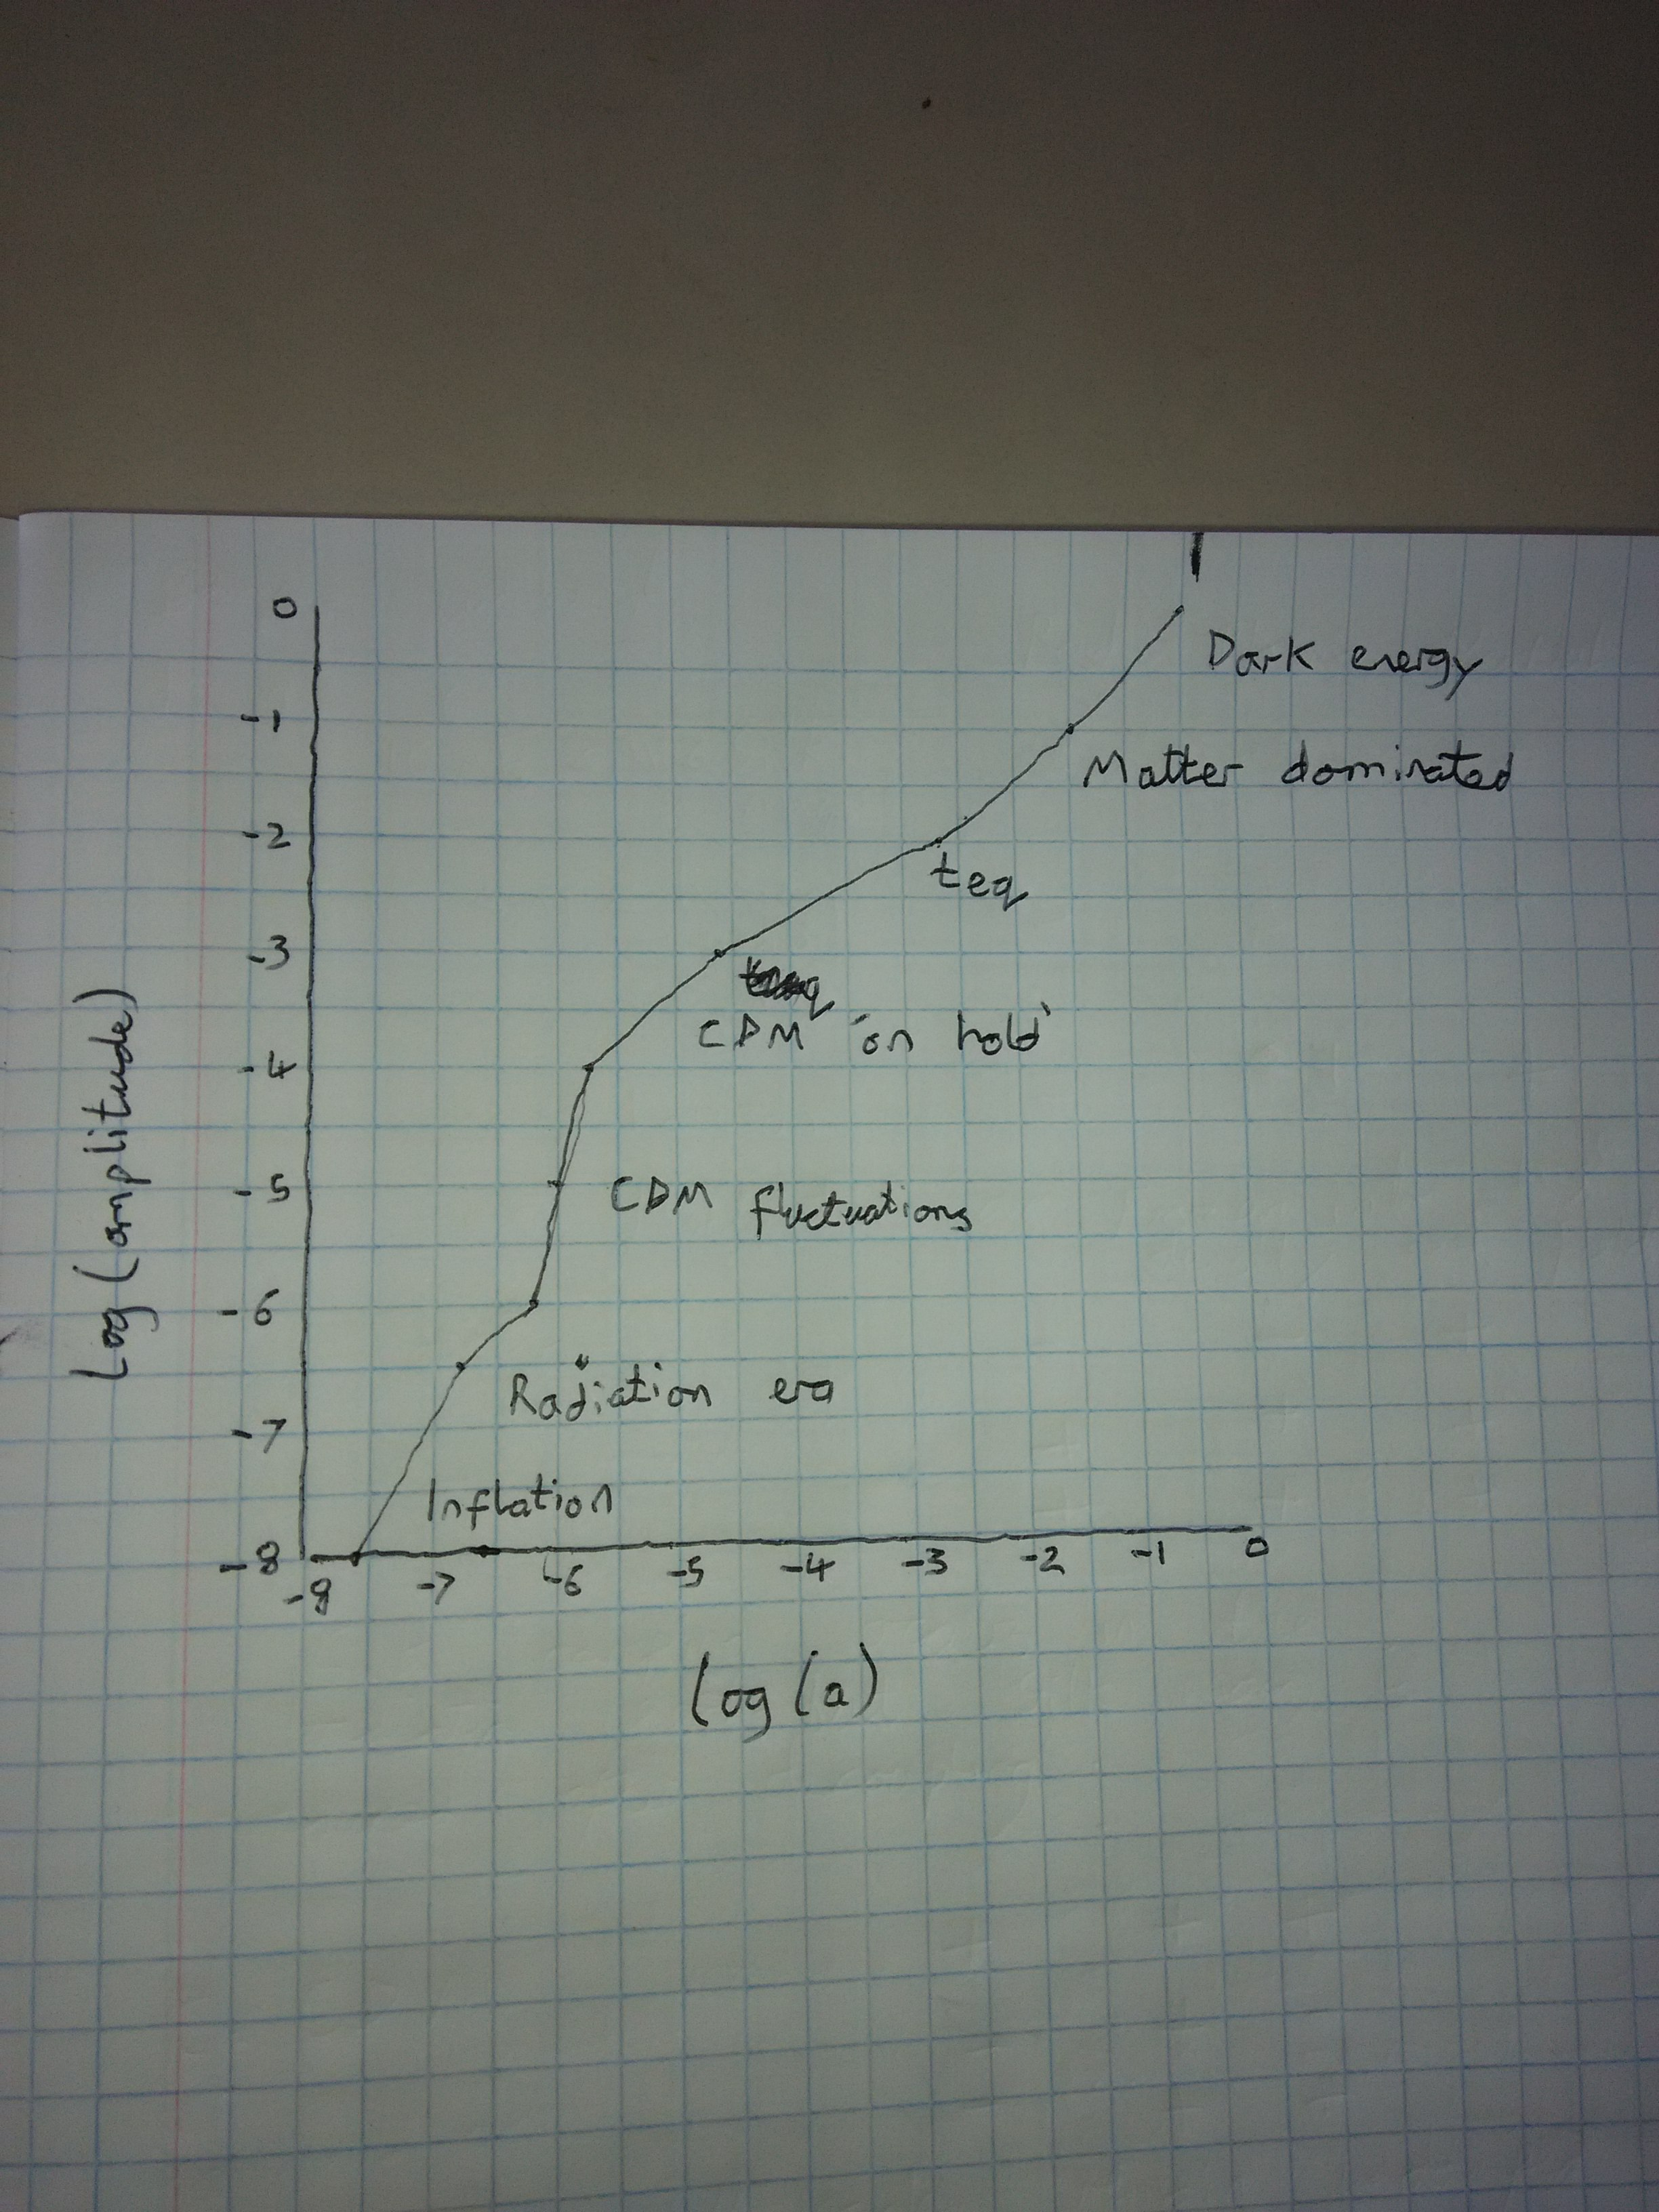
\includegraphics[width=.9\textwidth]{./tutorial9.jpg}
\caption{}
\label{fig:1}
\end{figure}
\section{}
Horizon problem - regions of the sky more than $1\degree (\approx 200Kpc)$ were never in causal contact before decoupling so no information could have
been exchanged. So why it is so isotropic?

Flatness problem - Why is $\Omega=1$ in universe today? The early universe must have had $\Omega=1$ as well (proof is in the notes).

Inflation solves the horizon problem because the causal horizon could have been larger in the past. Inflation also predicts that $\Omega=1$ because
size of universe was so large after inflation that any curvature would have been negligible.
\section{}
\begin{flalign*}
& K_0=1+.227N_{\nu} &\\
& N_{\nu}=3.046 &\\
& K_0=1.691 &\\
& 10^{-35}=1.691^{-\frac{1}{2}}\left(\frac{1.52\times10^{10}}{T}\right)^2 &\\
& \left(\frac{1.52\times10^{10}}{T}\right)^2=\frac{10^{-35}}{.769} &\\
& \frac{1.52\times10^{10}}{T}=\sqrt{1.3\times10^{-35}} &\\
& T=\frac{1.52\times10^{10}}{3.6\times10^{-18}} &\\
& T=4.22\times10^{27}K &\\
& kT=8.62\times10^{-5} eVK^{-1}\times 4.22\times10^{27}K &\\
& =3.64\times10^{23} eV &\\
& =3.64\times10^{14} GeV
\end{flalign*}
I couldn't answer the last bit.
%\begin{thebibliography}{1}
%\end{thebibliography}
\end{document} 